% !Mode:: "TeX:UTF-8"%確保文檔utf-8編碼
%新加入的命令如下: reduline showendnotes 
%新加入的环境如下:solution solutionorbox solutionorlines solutionordottedlines

\documentclass[12pt]{exam}%实际打印的时候加上twoside选项
\newlength{\textpt}
\setlength{\textpt}{12pt}

\usepackage{teachingplan}
\usetikzlibrary{patterns,calc}

%写上答案或者不写上答案%
\printanswers  


%讲知识点然后测试,测试通过继续下一个知识点。不通过给予小提示,然后继续测试,如果通过那么通过,如果还是不会做,那么继续讲解知识点,并讲解这个题目,然后重新给出一个题目重新测试。

%如果有精力,后面再准备一套中考真题。

%\excludecomment{knowledge}
\includecomment{knowledge}
\excludecomment{Aquestions}
%\includecomment{Aquestions}

\begin{document}
\begin{coverpages}
\title{压强}
\author{德山书生}
\maketitle
\tableofcontents
\end{coverpages}
\begin{knowledge}
\begin{flushright}
\begin{notecard}{12em}
\ttfamily
重要的不是正确答案,而是明白自己对在那里。
\end{notecard}
\end{flushright}
\section{压强}
垂直压在物体表面上的力叫\answerline*[压力]。压力的方向垂直于受力面。

压力的作用效果由压力和\answerline*[受力面积]共同决定。

物体\answerline*[单位面积]上受到的压力叫做压强,用符号$p$表示。

压强的计算公式是:
\begin{solutionorbox}[6ex]
$\textrm{压强}(p)=\frac{\textrm{压力}(F)}{\textrm{受力面积}(S)}$
\end{solutionorbox}

压强的单位是帕斯卡,简称\answerline*[帕],用符号Pa表示,1Pa=1\si{N/m^2}


\textbf{问题:}如图所示,用100N的水平力将9N的物体压在竖直的墙上,物体和墙壁的接触面积为\si{100cm^2},则物体对墙壁的压强为(\answerline*[B])。
\begin{multicols}{2}
\begin{figure}[H]
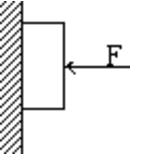
\includegraphics[scale=1]{图1}
\end{figure}
\columnbreak
\begin{choices}
\choice  900Pa 
\choice  \num{1d4} Pa
\choice \num{9.8d5} Pa 
\choice \num{1.09d4} Pa 
\end{choices}
\end{multicols}


由压强公式可知改变压强大小方法有:
\begin{solutionorbox}[8ex]
①减小压力或增大受力面积,可以减小压强;②增大压力或减小受力面积,可以增大压强。
\end{solutionorbox}


\textbf{(2012北京,7,2分)}下列实例中,目的是为了增大压强的是(\answerline*[A])
\begin{choices}
\begin{multicols}{2}
\choice 刀刃做得很薄
\choice 书包带做得较宽
\columnbreak
\choice 坦克装有宽大的履带
\choice 大型平板拖车装有很多轮子
\end{multicols}
\end{choices}

\textbf{(2013湖北宜昌,23,2分)}小华质量为50kg,每只脚与地面的接触面积为200\si{cm^2},他双脚站立时对水平地面的压强为\numb{1.25d4}\si{Pa},他走路时对水平地面的压强会\answerline*[变大](“变大”、“变小”或“不变”)。($g$=10N/kg)



\textbf{(2012上海,8,2分)}如图所示,放在水平地面上的物体$A$、$B$高度相等,$A$对地面压力小于$B$对地面的压力。若在两物体上部沿水平方向切去相同的厚度,则切去部分的质量${m_A}^{'}$、${m_B}^{'}$的关系是(\answerline*[C])
\begin{multicols}{2}
\begin{choices}
\choice ${m_A}^{'}$一定大于${m_B}^{'}$
\choice ${m_A}^{'}$可能大于${m_B}^{'}$
\choice ${m_A}^{'}$一定小于${m_B}^{'}$
\choice ${m_A}^{'}$可能等于${m_B}^{'}$
\end{choices}
\columnbreak
\begin{fig}{2012上海8}
\end{fig}
\end{multicols}


\begin{fig}{2012上海8解说}
\label{fig:2012上海8解说}
\end{fig}
解说:对于固体形状规则近似的有$p=\rho gh$,则有$F=\rho ghS$,在底面积不变密度均匀的情况下,我们有$F\propto h$,那么就类似的有上面的图形,每增加一点点小片h,物体对地面的压力是这样正比例增加的。所以之前$A$比$B$的压力要小,后面切出的那部分同样对地面的压力要小,所以质量要小。(这里为了读者方便理解,我说得很详细,整个思维过程在解题时一扫而过会很快的。)


\section{液体的压强}
液体的压强是由于液体受到\answerline*[重力]而产生的,由于液体具有流动性,对器壁也产生了压强。

液体压强大小的规律:
\begin{enumerate}
\item[①] 同一深度处,各个方向上压强大小\answerline[相等]
\item[②] 深度越大,压强也\answerline[越大]
\item[③] 不同液体同一深度处,液体密度大的,压强\answerline[也大]。[深度h,液面到液体某点的\textbf{竖直}高度。]
\end{enumerate}


液体压强的计算公式是?并请说明单位和常数:
\begin{solutionorbox}[8ex]
$p=\rho gh$ 。$\rho$指该液体的密度,单位\si{kg/m^3},$g$=9.8N/Kg,$h$指到液面的垂直深度,单位:m。
\end{solutionorbox}

由液体压强公式可知液体的压强只与液体的密度和所处的\answerline*[深度]有关。


\textbf{(2012四川成都A,6,2分)}下列说法正确的是(\answerline*[C])
\begin{choices}
\choice 液体内部没有压强
\choice 液体对容器底部有压强,对容器侧壁没有压强
\choice 液体内部同一深度处,各个方向压强相等
\choice 液体压强与深度有关,与液体密度无关
\end{choices}


\subsection{液体压强的两种算法}
液体压强现在有两种算法了,$p=FS$和$p=\rho gh$,那么什么时候用什么算法呢?请看下题:\\
\textbf{问题:}如下图所示的水桶中,存水10N,水深8cm,水桶的底面积是\si{100cm^2},则桶底所受水的压强为\answerline*[800]Pa,桶底所受水的压力为\answerline*[8]N\\。($g$取10N/kg)
\begin{figure}[H]
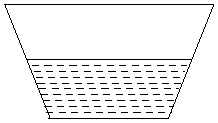
\includegraphics[scale=1.5]{水桶}
\end{figure}



\subsection{对正比例的反思}
在上面题目2012上海8的解说中\ref{fig:2012上海8解说},我们提到了规则形状固体的压力和高度h在密度和底面积不变的情况下成正比例这个事实,并通过作图更直观的感受这一事实,而对于液体,则这一规律是\uwave{一定成立}的。现在让我们用这一思路来看下面这个题目。

\textbf{(2011上海,7,2分)[难]}如图所示,底面积不同的圆柱形容器$A$和$B$分别盛有甲、乙两种液体,两液面相平且甲的质量大于乙的质量。若在两容器中分别加入原有液体后,液面仍保持相平,则此时液体对各自容器底部的压强$p_A$、$p_B$和压力$F_A$、$F_B$的关系是(\answerline*[D])
\begin{multicols}{2}
\begin{linefig}{2011上海7}
\end{linefig}
\columnbreak
\begin{choices}
\choice $p_A<p_B$、$F_A=F_B$
\choice $p_A<p_B$、$F_A>F_B$
\choice $p_A>p_B$、$F_A=F_B$
\choice $p_A>p_B$、$F_A>F_B$
\end{choices}
\end{multicols}

我们可以看到用这种图形正比例思路可以快速判断出$F_A>F_B$,那么对于压强的分析你们会了吗?

我们看到$p=\rho gh$这个公式对于液体和形状竖直方向规则的固体(比如圆柱体,长方体等)都是成立的。现在用两个题目检验一下:

\textbf{问题:}如图所示,三个材料相同,但

\subsection{连通器}
上端开口,下部连通的容器叫连通器。连通器里的液体不流动时,各容器中的液面高度总是\answerline*[相同]的。



\section{大气压强}
大气对浸在它里面的物体的压强叫大气压强,简称大气压或气压。大气压是由于气体受重力且具有流动性而产生的。

\subsection{托里拆利实验}
测定大气压强数值的是托里拆利(意大利科学家)。托里拆利管倾斜后,水银柱高度\answerline*[不变],长度\answerline*[变长]。

$1$个标准大气压=$76$厘米水银柱高=$1.01 \times 10^5$帕\leftnote{如果是水呢?}

问题:如果管子变粗会如何呢?如果管子提上一点提下一点会如何呢?如果做实验不小心上面混入一点空气会如何呢?

反向思考,如果已知大气压强,我们是不是可以类似的算出某个未知液体的密度。

\begin{questions}
\setcounter{question}{2}
\question
某同学在标准气压下做托里拆利实验,测得的结果是管内水银面比槽里水银面高出了$750mm$,他失败的原因是:(\answerline*[D])
\begin{choices}
\choice 管子粗了一些
\choice 管子长了一些
\choice 管子不在竖直位置
\choice 管内漏入少量空气
\end{choices}

\question
托里拆利实验中,若在玻璃管顶开一小孔,则管内水银将:(\answerline*[C])
\begin{choices}
\choice 往上喷出
\choice 保持高度不变
\choice 降到与管外水银面相平
\choice 稍下降一些
\end{choices}
\end{questions}


\subsection{马徳堡半球实验}
马徳堡半球实验既证明了大气压强的存在也证明了真空的存在。说明马徳堡半球实验的近似处理方法。

\begin{questions}
\setcounter{question}{4}
\question
(2012年湖北省宜昌市中考物理试题)\\
在德国马德堡市的广场上,1654年曾经做过一个著名的马德堡半球实验,如下图左所示,把两个半径约$20cm$的铜制空心半球合在一起,抽去里面的空气,用两支马队向相反的方向拉两个半球。 
\begin{figure}[H]
\centering
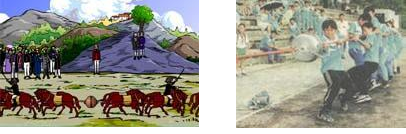
\includegraphics[width=\linewidth]{图3}
\end{figure}

(1)总共用了16匹马把两个半球拉开,则平均一对(左右各一匹)马产生的拉力是多少?(大气压的值约为$10^5$Pa,计算时把半球看成一个圆盘。) 
\begin{solutionorbox}[8ex]
大气压产生的压力:$F=PS=10^5Pa \times 3.14 \times (0.2m)^2=12560N$, 一对马产生的拉力: 
F拉=1570N。
\end{solutionorbox}

(2)某实验室供教学用的半球,在正常气压下抽成真空后,只需四个人便可拉开。其原因是\shortanswerline 。
\begin{solutionorbox}[6ex]
半球表面积较小(或半径小、或体积较小),产生的大气压力小。 
\end{solutionorbox}

(3)如上图右是同学们用高压锅模拟马德堡半球实验,如果他们没有抽气机,应怎样将高压锅里的空气尽量排除呢?请说出你的办法\shortanswerline 。
\begin{solutionorbox}[10ex]
在高压锅中放少量的水,盖上锅盖,加热至沸腾,让水蒸气将空气赶出高压锅,此时将限压阀罩上,然后向高压锅上泼冷水,使锅中的水蒸气遇冷液化,锅中就几乎没有空气了。
\end{solutionorbox}
\end{questions}

\subsection{大气压的应用}
大气压的应用:活塞式抽水机和离心式抽水机。问题:抽水机最高抽多高?

\section{流体压强和流速的关系}
流体(气体和液体)流动时,流速越大的位置压强越\answerline*[小]。\leftnote{飞机机翼分析}
%\endnote{风洞的试验结果或电脑的模拟运算都显示:机翼顶部的气流要比底部的气流快很多到达机翼后沿。合理的解释除了伯努利效应外还有康达效应并通过牛顿第三定律起的作用。参考网站:http://www.ied.edu.hk/apfslt/v5\_{}issue1/ngph/}


\end{knowledge}



\begin{Aquestions}
\newpage
\section{题库A}
\begin{questions}
\question
在一些公共汽车上配备逃生锤,遇到紧急情况时,乘客可以用逃生锤打破玻璃逃生,为了更容易打破玻璃,逃生锤外形应选择下面的(\answerline*[C])
\begin{choices}
\begin{multicols}{4}
\choice 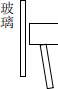
\includegraphics[scale=1]{figures/图片1-1.png} 
\columnbreak
\choice 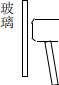
\includegraphics[scale=1]{figures/图片1-2.png} 
\columnbreak
\choice 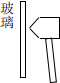
\includegraphics[scale=1]{figures/图片1-3.png} 
\columnbreak
\choice 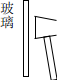
\includegraphics[scale=1]{figures/图片1-4.png} 
\end{multicols}
\end{choices}

\question
如下图所示,液体压强使坝底的水喷射而出,那么决定坝底水的压强大小的是(\answerline*[C])
\begin{multicols}{2}
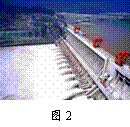
\includegraphics[scale=1]{figures/图片2.png} 
\columnbreak
\begin{choices}
\choice 坝的宽度
\choice 水的体积
\choice 水的深度
\choice 坝的高度
\end{choices}
\end{multicols}


\question
下图所示的四个实例中,为了增大压强的是(\answerline*[C])

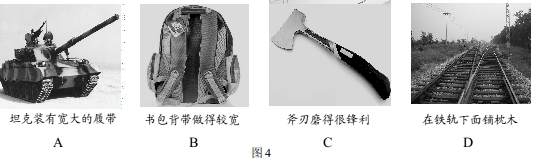
\includegraphics[scale=1]{figures/图片4.png} 


\question
下列现象中,为了增大压强的是(\answerline*[D])
\begin{choices}
\choice 骆驼长着宽大的脚掌
\choice 载重汽车装有许多轮子
\choice 坦克车装有宽宽的履带
\choice 压路机装有质量很大的碾子
\end{choices}


\question
小华想用空易拉罐来证明大气压强的存在,下列操作能达到目的的是(\answerline*[D])
\begin{choices}
\choice 用手捏空易拉罐,易拉罐变瘪
\choice 将易拉罐密封后置于深水中,易拉罐变瘪
\choice 让空易拉罐从高处下落撞击地面, 易拉罐变瘪
\choice 用注射器抽取密封易拉罐中的空气,易拉罐变瘪
\end{choices}


\question
如下图所示,用两食指同时压铅笔两端,左手指受到的压力为F1,压强为P1,右手指受到的压力为F2,压强为P2,下列说法中正确的是(\answerline*[C])
\begin{multicols}{2}
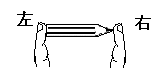
\includegraphics[scale=1]{figures/图片7.png} 
\columnbreak
\begin{choices}
\choice F1<F2
\choice F1>F2
\choice P1 <P2
\choice P1>P2
\end{choices}
\end{multicols}


\question
李老师经常引导学生利用身边的生活用品做实验,通过动手动脑,学习物理知识,揭示物理规律。下图的实验中不是揭示流体压强与流速关系的是(\answerline*[C])

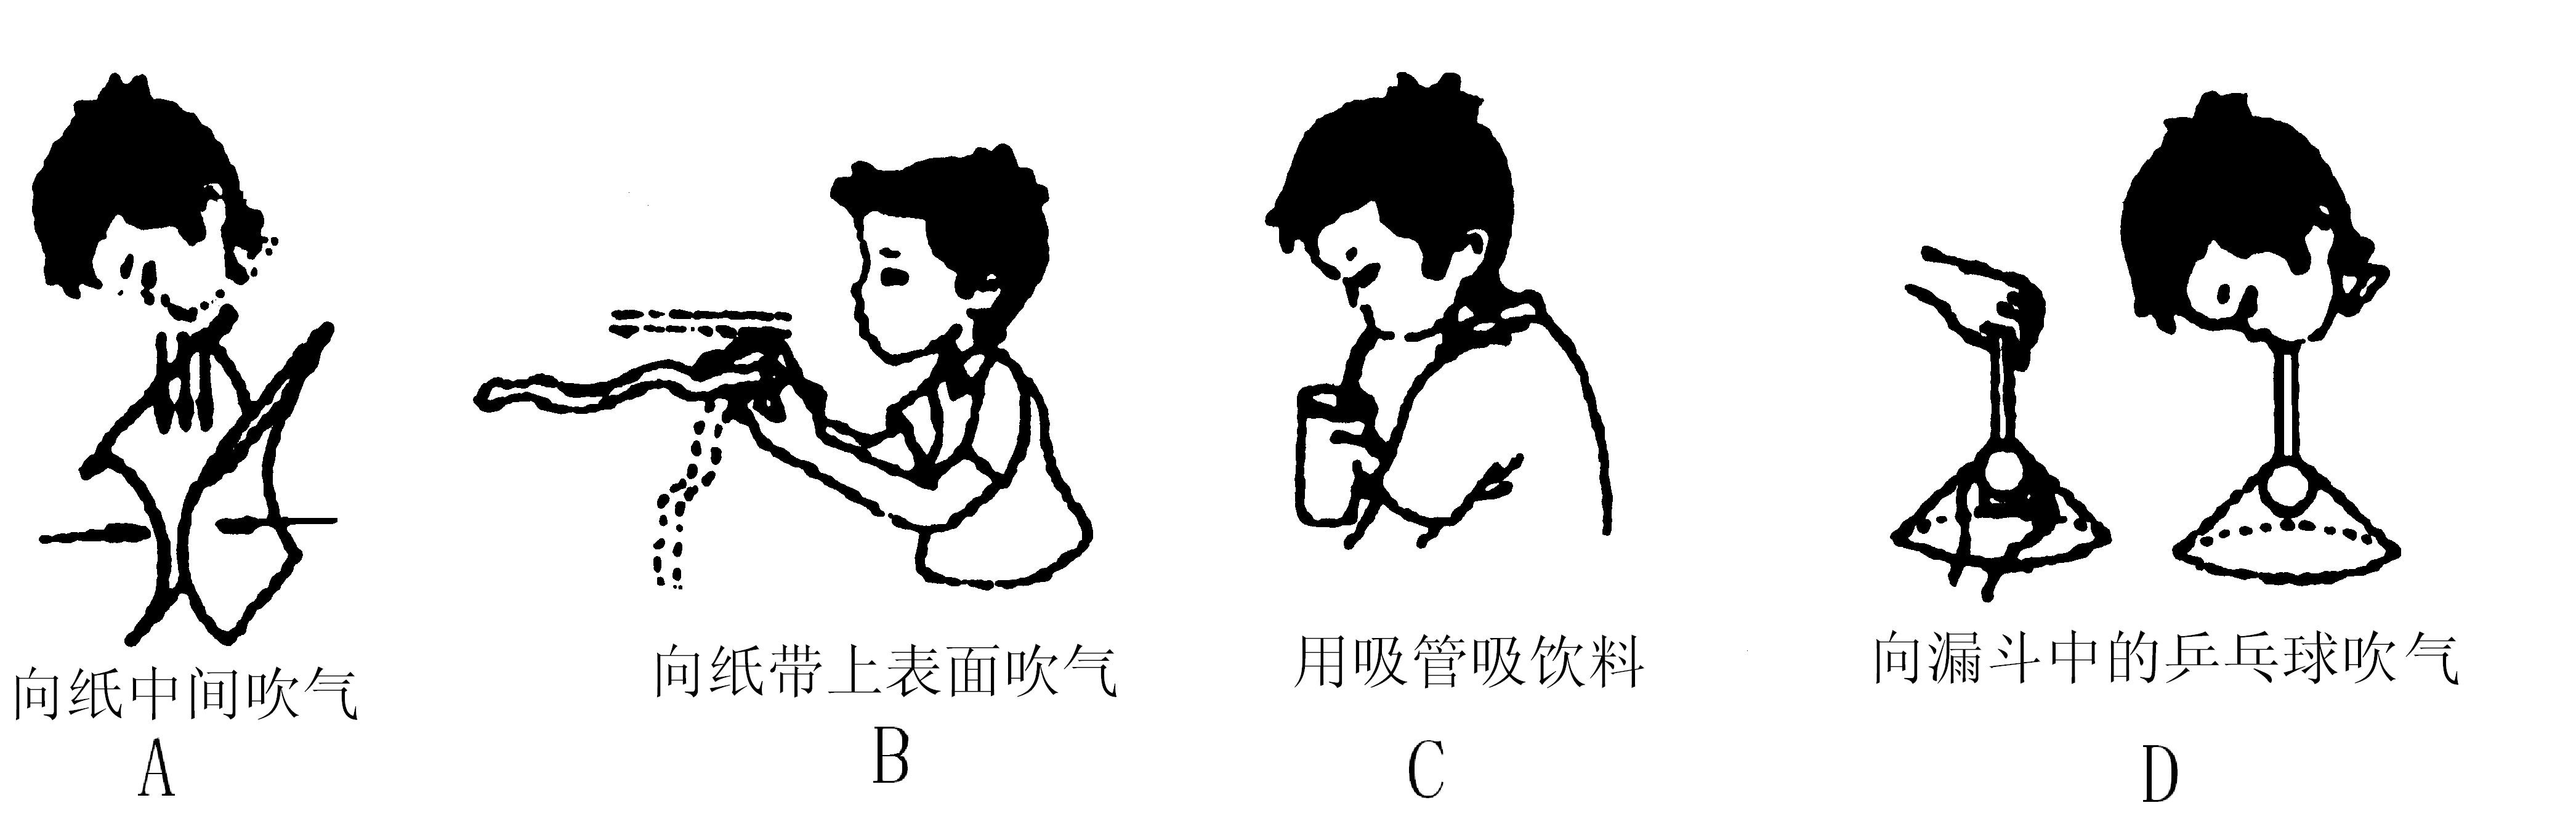
\includegraphics[width=\linewidth]{figures/图片8.png} 


\question
如下图所示,同样的木块在盛有不同液体的容器中保持静止,四个容器中的液面到容器底面的距离相同,则容器底面受到的液体压强最大的是(\answerline*[A])

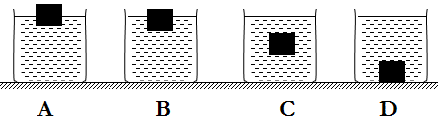
\includegraphics[scale=1]{figures/图片9.png} 


\question
如下图所示,在倒置的透明漏斗里放置一个乒乓球,用手指托住乒乓球,松手后,乒乓球受重力作用将下落;若向倒置的漏斗用力吹气再松手时,乒乓球不但没有被吹下去,反而被“吸”住了。这是因为乒乓球上方空气的流速\answerline*[大于] (填“大于”、“小于”或“等于”)其下方空气的流速,依据流速越大的位置压强越\answerline*[小]的原理,乒乓球受压强差的作用而不下落。

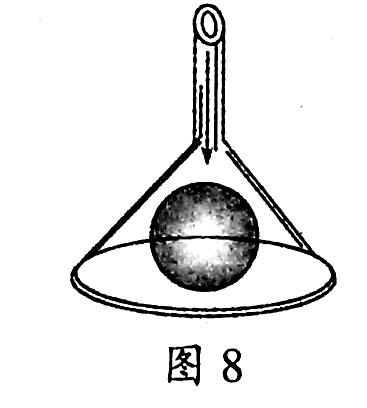
\includegraphics[scale=0.2]{figures/图片10.jpg} 


\question
如下图所示的实例中,目的是为了增大压强的是(\answerline*[C])

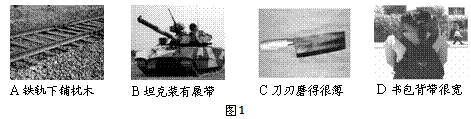
\includegraphics[scale=1]{figures/图片+1.png} 


\question
如下图所示,当试管从倾斜放置到竖直放置的过程中,水对试管底部的压强(\answerline*[A])
\begin{multicols}{2}
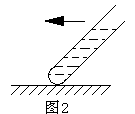
\includegraphics[scale=1]{figures/图片+2.png} 
\columnbreak
\begin{choices}
\choice 变大
\choice 不变
\choice 变小
\choice 无法确定
\end{choices}
\end{multicols}


\question
如下图所示,完全相同的两块砖分别平放和立放在水平地面上,已知砖的长:宽:高为4:2:1,若砖平放时对地面的压强为P1;立放时对地面的压强为P2,则P1:P2等于(\answerline*[C])
\begin{multicols}{2}
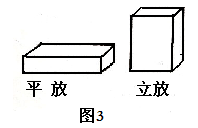
\includegraphics[scale=1]{figures/图片+3.png} 
\columnbreak
\begin{choices}
\choice 8:1
\choice 4:1
\choice 1:4
\choice 1:8
\end{choices}
\end{multicols}


\question
高度、材料相同的实心长方体A和B放在水平桌面上,它们的大小如下图所示。它们对桌面的压力分别为FA,FB;压强分别为PA、PB。关于它们的大小关系,正确的是(\answerline*[B])
\begin{multicols}{2}
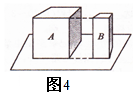
\includegraphics[scale=1]{figures/图片+4.png} 
\columnbreak
\begin{choices}
\choice FA<FB   PA<PB
\choice FA>FB   PA=PB
\choice FA>FB   PA>PB
\choice FA>FB    PA<PB
\end{choices}
\end{multicols}


\question
下图中的推土机有宽大的履带和锋利的土铲,下列说法正确的是(\answerline*[D])
\begin{multicols}{2}
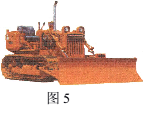
\includegraphics[scale=1]{figures/图片+5.png} 
\columnbreak
\begin{choices}
\choice 宽大的履带是为了减小压力
\choice 宽大的履带是为了增大压强
\choice 锋利的土铲是为了减小压力
\choice 锋利的土铲是为了增大压强
\end{choices}
\end{multicols}


\question
一块质量为$7.9kg$的实心正方体铁块,放在一个长与宽分别为$40cm$和$20cm$的长方形水平桌面中央,则水平桌面对铁块的支持力为\answerline*[79N],铁块对水平桌面的压强为\answerline*[7900Pa]($\rho _\textrm{铁}=7.9 \times 10^3 kg/m^3 , g=10N/kg$)。

\question
一瓶“娃哈哈”饮用纯净水上标有“$569ml$”的字样,则水的质量为\\ \answerline*[0.569]kg。如果测得瓶底与水平桌面的接触面积为$5cm^3$,这瓶水对桌面的压强为\answer[60pt]{$1.138 \times 10^4$}Pa(忽略瓶的质量,水的密度$\rho _\textrm{水}=1.0 \times 10^3 kg/m^3$,取$g=10N/kg$)。


\question
用吸管从瓶子中吸饮料时,是\answerline*[大气压]力使饮料上升到嘴里。离地面越高的地方,那里的大气压强越\answerline*[小]。


\question
医生把注射器针头插入药水瓶,把注射器活塞往外拉时,药液在\answerline*[大气压]的作用下进入注射器内。注射器针头做得比较尖,这是为了\answerline*[增大压强]。


\question
小明制作了如下图所示的潜艇模型。当把模型中的空气吸出时,模型就能下沉。模型在下沉过程中所受到水的压强\answerline*[增大](选填“减小”、“不变”或“增大”);当模型沉到距水面$0.2m$处时,模型受到水的压强大小为\answerline*[2000]Pa。


\question
小红同学手拿着几条轻而软的小彩带站在公路边,突然一辆小汽车从她旁边高速驶过,这时发现小彩带往公路内飘起来,如下图所示,请用所学过的物理知识解释这种现象。
\begin{multicols}{2}
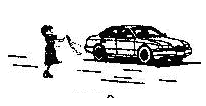
\includegraphics[scale=1]{figures/图片+11.png} 
\columnbreak
\begin{solution}[16ex]
当小汽车高速驶过时,公路一侧气流速度增大(1分),压强变小(1 分),公路外侧气流速度较小,压强较大(1分),小彩带因这个压强差,会受到一个从公路外侧指向公路内侧的压力作用而飘起来(1分)。
\end{solution}
\end{multicols}


\question
夏日的北海银滩,游客在水平沙滩上驾驶四轮沙滩摩托车,摩托车和人的总重约为$3.2 \times 10^3 N$,每个车轮与沙地的接触面积约为$0.02m^2$。问:
\begin{multicols}{2}
(1)摩托车对沙地的压力是多大?\\
(2)摩托车对沙地的压强是多大?\\
(3)沙滩摩托车的车轮比普通摩托车的车轮要大得多,这样设计车轮有什么好处(写出一点即可)?  
\columnbreak
\begin{center}
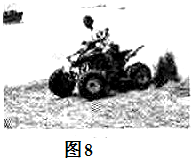
\includegraphics[scale=0.9]{figures/图片+12.png}
\end{center}
\end{multicols}

\begin{solution}[18ex]
(1)摩托车对沙地的压力为$F=G_\textrm{总}=3.2\times 10^3N$\\
(2)摩托车与沙地的接触面积为$S=4\times 0.02m^2=0.08m^2$,则摩托车对沙地的压强为
\begin{equation*}
p=\frac{F}{S}=\frac{3.2\times 10^3 N}{0.08m^2}=4\times 10^4 Pa
\end{equation*}
(3)在压力相等的情况下增大了受力面积,可以减小沙滩摩托车对沙地的压强,使车轮不易陷入沙子里。(答案中涉及减小压强但无“压力相同”的条件只得1分)
\end{solution}


\end{questions}
\end{Aquestions}



%\section{小信息}
%\showendnotes


\end{document}



